% Created 2025-05-06 Tue 14:19
% Intended LaTeX compiler: pdflatex
\documentclass[11pt]{article}
\usepackage[utf8]{inputenc}
\usepackage[T1]{fontenc}
\usepackage{graphicx}
\usepackage{longtable}
\usepackage{wrapfig}
\usepackage{rotating}
\usepackage[normalem]{ulem}
\usepackage{amsmath}
\usepackage{amssymb}
\usepackage{capt-of}
\usepackage{hyperref}
\synctex=1
\usepackage[margin=1in]{geometry}
\usepackage{graphicx}
\usepackage{amsmath,bm}
\usepackage{algpseudocode}
\usepackage[ruled,vlined]{algorithm2e}
\usepackage[version=4]{mhchem}
\usepackage{siunitx}
\usepackage{longtable,tabularx}
\usepackage{booktabs}
\usepackage{tabularx,longtable,multirow,subfigure,caption}
\setlength\LTleft{0pt}
\usepackage{mathrsfs}
\usepackage{amsfonts}
\usepackage{enumitem}
\usepackage{mathalpha}
\usepackage{setspace}
\onehalfspacing
\author{Alvaro Cea\footnote{Research Associate, CAGB 308, South Kensington Campus. (alvaro.cea-esteban15@imperial.ac.uk)}, Rafael Palacios\footnote{Professor in Computational Aeroelasticity, CAGB 310, South Kensington Campus. AIAA Associate Fellow (r.palacios@imperial.ac.uk)}}
\date{}
\title{Differentiable and Nonlinear Aircraft Loads at Large Scale Using an Accelerator-Based Concurrent Solution}
\hypersetup{
 pdfauthor={Alvaro Cea\footnote{Research Associate, CAGB 308, South Kensington Campus. (alvaro.cea-esteban15@imperial.ac.uk)}, Rafael Palacios\footnote{Professor in Computational Aeroelasticity, CAGB 310, South Kensington Campus. AIAA Associate Fellow (r.palacios@imperial.ac.uk)}},
 pdftitle={Differentiable and Nonlinear Aircraft Loads at Large Scale Using an Accelerator-Based Concurrent Solution},
 pdfkeywords={},
 pdfsubject={},
 pdfcreator={Emacs 29.4 (Org mode 9.6.15)}, 
 pdflang={English}}
\begin{document}

\maketitle

\begin{abstract}
A novel framework for geometrically nonlinear aeroelastic analysis is augmented for large scale computations of aircraft-sizing loads. The software can be deployed on modern hardware architectures and the parallelisation has been tested both on CPUs and GPUs. While keeping computational times in the order of seconds, the presented approach unlocks new capabilities such as the following: uncertainty quantification analysis of the nonlinear response via massively-parallel Montecarlo simulations; construction of load envelopes of static and dynamic cases in full-aircraft models. Furthermore, differentiation of both Montecarlo simulations and load is achieved via JAX library automatic differentiation engine and collective primitives. 
We explore a high-aspect-ratio-wing aircraft configuration, showing the ability of the solvers to capture nonlinear effects for external forces inducing large deformations and also the importance of these effects when studying modern aircraft concepts. Discrete, manoeuvre and gust loads are assessed for multiple flow and parametric conditions running concurrently. Sensitivities of maximum wing stresses in the load-envelopes are computed and verified against finite differences.  
\end{abstract}


\section{Introduction}
\label{sec:orgace15ff}
Aeroelastic analysis are expected to become critical in the very early phases of the wing design process: while the field was more important in post-design stages to ensure in-flight integrity, it now becomes paramount to capture the cross-couplings between disciplines. 
As highlighted in \cite{LIVNE2018}, formulations that include nonlinear effects should be developed that not only enhance current modelling techniques  but that also allow rapid data turnaround for the industry. Real-time, hardware-in-the-loop flight simulators would also benefit of actively controlled, deformable airplane models. This leads to a more nonlinear landscape, where the overall aerodynamic performance needs to be calculated around a flight shape with large deformations \cite{JONSSON2023}; the input for efficient control laws account for the steady state and nonlinear couplings \cite{Artola2021}; and the loads ultimately sizing the wings are atmospheric disturbances computed in the time-domain \cite{CESNIK2014}.
A more holistic approach to the design also increases the complexity of the processes exponentially, and the trade-offs and cost-benefit analysis may not be possible until robust computational tools are in-place to simulate the different assumptions.
 Certification of new air vehicles is another important aspect that requires 100,000s of load cases simulations \cite{Kier2017}, as it considers manoeuvres and gust loads at different velocities and altitudes, and for a range of mass cases and configurations. This poses another challenge for new methods that aim to include new physics since they normally incur in prohibitively expensive computational times. 
Lastly, the mathematical representation of the airframe, embodied in the complex Finite-Element Models (FEMs) built by organizations, encompasses a level of knowledge that is to be preserved when including the new physics mentioned above. 
\\[0pt]
Those previous considerations set the goals for our  work: 1) to be able to perform geometrically nonlinear aeroelastic analysis, 2) to work with existing generic FEMs in a non-intrusive manner, and 3) to achieve a computational efficiency that is equivalent to present linear methods (if not faster). 1) and 2) were considered in \cite{CEA2023,CEA2024}. 
In this work we explore the latest advances on accelerator's parallelisation and how to integrate them into our solution process to enable large scale aeroelastic simulations under geometrically nonlinear assumptions.
Specifically, we set out to characterise the dynamics of highly flexible aircraft in response to the very large envelopes of in-flight loads encountered in the certification process. 
For that purpose, we have leveraged the numerical library JAX \cite{jax2018github} to build a new simulation environment for time-domain nonlinear aeroelastic analysis that achieves two orders of magnitude speed-ups with respect to standard implementations \cite{CEA2024},  is suitable for modern hardware architectures such as GPUs \cite{ALVAROCEA2024}, and that is also capable of computing derivatives via algorithmic differentiation \cite{ALVAROCEA2024a}. The strength and suitability of JAX for scientific computation has been proved recently in fluid dynamics \cite{BEZGIN2023} and solid mechanics \cite{XUE2023} applications. 
We want to go one step further by adding parallelisation and distributed computational capabilities to the codebase to tackle the very demanding task of calculating load envelopes while introducing new physics to account for the large displacements and rotations ultra-high-aspect-ratio wings undergo. 
In this multi-process environment, a Single Program Multiple Data (SPMD) paradigm is employed with the main computation spanning as many devices as available in the cluster and performing collective operations to communicate between devices. 
By addressing in one program a substantial part of scenarios during flight (manoeuvres and gust responses at different velocities and altitudes, and for a range of mass cases and configurations), we will be able to produce the critical loading characteristics of the aircraft at a fraction of time. Moreover, as future work we aim to differentiate the boundaries of these critical cases  using the already demonstrated capabilities AD, thereby providing gradients for optimization studies as well as additional insights to the designer.  
\\[0pt]
The paper is organised as follows: Sec. \ref{sec:org85f0cd2} gives and overview of the theoretical and computational developments that underpin this work with a focus on the new parallelisation capabilities. In sec. \ref{sec:org0a86af3}, a representative configuration of an ultra-high-aspect-ratio aircraft is studied under various loading scenarios that have been parallelised; namely structural static loads, manoeuvre cases for varying flow conditions and dynamic loads with multiple gusts running concurrently. This application of modern hardware architectures to aircraft nonlinear load analysis is novel and could potentially be introduced inside current industrial processes. We conclude in Sec. \ref{sec:orgb486577} with a summary of the main advances and the future work that is needed to finalise a formulation that may run in parallel on modern hardware architectures as well as being differentiated.  
\section{Theoretical and computational background}
\label{sec:org85f0cd2}
The main aspects of the aeroelastic framework we have developed are presented in this section. 
The approach is built on a non-intrusive reduction order process combined with a nonlinear description of the dominant dimension for slender structures. It achieves a nonlinear representation of aeroelastic models of arbitrary complexity in a very efficient manner and without losing the characteristics of the linear model. We target the calculation of flight loads herein, but it can also be applied to the computation of aeroelastic stability phenomena such as flutter or divergence \cite{CEA2023} and to broader multidisciplinary design optimisation problems, which are currently being explored.
The key features of the formulation are:

\begin{itemize}
\item Geometrically nonlinear aeroelastic analysis using complex GFEMs: achieved via a three step process in which a condensed model is first produced, the dynamics of this reduced model are described by a system on nonlinear equations \cite{HODGES2003} written in material velocities and stresses, and a modal expansion of those variables is the final key step in seamlessly mapping the global FEM into the nonlinear description \cite{PALACIOS2011}. The overall process can be found in \cite{CEA2021a}.
\item Maximum performance: as a combination of a highly optimised and vectorised codebase, numerical library JAX with its JIT compiler and accelerator capabilities  driving the calculations, and the newly added added parallelisation of load cases.
\item Differentiation and sensitivity analysis: using JAX algorithmic differentiation toolbox, the entire process, from inputs to aeroelastic outputs can be differentiated \cite{CEA2024a}.
\end{itemize}

\subsection{Nonlinear aeroelastic system}
\label{sec:org382dc9e}
Given a general GFEM, a reduced model is obtained from a static or dynamic condensation that captures well the stiffness and inertia properties in the condensed matrices, \(\pmb{K}_a\) and \(\pmb{M}_a\). The eigenvalue solution of the FEM yields the modal shapes, \(\pmb \Phi_0\), and frequencies \(\pmb \omega\). A projection of the state variables, velocities \(\pmb{x}_1 = \pmb{\Phi}_1\pmb{q}_1\) and stresses \(\pmb{x}_2 = \pmb{\Phi}_2\pmb{q}_2\), and a Galerkin projection of the equations of motion leads to the system of ODEs that is solved in time domain. 
Aerodynamic forces are obtained via Generalised Aerodynamic Forces (GAFs) using a panel-based DLM solver and Roger's rational function approximation\cite{Roger1977} to bring the forces to the time domain, resulting in a modal force component given as:

\begin{equation}\label{eq3:eta_full}
\begin{split}
\bm{\eta}_a = Q_\infty & \left(\vphantom{\sum_{p=1}^{N_p}} \pmb{\mathcal{A}}_0\bm{q}_0 +b\pmb{\mathcal{A}}_1 \bm{q}_1 +b^2 \pmb{\mathcal{A}}_2\dot{\bm{q}}_1    + \pmb{\mathcal{A}}_{g0}\bm{v}_g +b\pmb{\mathcal{A}}_{g1} \dot{\bm{v}}_g +b^2 \pmb{\mathcal{A}}_{g2}\ddot{\bm{v}}_g +  \sum_{p=1}^{N_p} \pmb{\lambda}_p  \right) 
\end{split}
\end{equation}
where the \(\pmb{\mathcal{A}}_is\) are real matrices, \(b=\frac{c}{2U_\infty}\) with \(c\) the reference chord, \(Q_\infty = \tfrac12\rho_\infty U_\infty^2\) the dynamic pressure, \(\pmb{\lambda}_p\) the aerodynamic states and \(N_p\) the number of lags. Note these forces naturally follow the structure since the formulation is written in the material frame of reference. 
The coupling of the structure and aerodynamic equations combined with the aerodynamic lags, gravity forces, \(\bm{\eta}_g\), and gust disturbances, \(\bm{v}_g\), gives the final ODE system: 
\begin{equation}
\label{eq2:sol_qs}
\begin{split}
\dot{\pmb{q}}_{1} &=  \hat{\pmb{\Omega}}  \pmb{q}_{2} - \hat{\pmb{\Gamma}}_{1} \pmb{:} \left(\pmb{q}_{1} \otimes \pmb{q}_{1} \right) - \hat{\pmb{\Gamma}}_{2} \pmb{:} \left( \pmb{q}_{2} \otimes  \pmb{q}_{2} \right) + \hat{\bm{\eta}}  \\
\dot{\pmb{q}}_{2} &= -\pmb{\omega} \odot \pmb{q}_{1} + \pmb{\Gamma}_{2}^{\top} \pmb{:} \left( \pmb{q}_{2} \otimes  \pmb{q}_{1} \right) \\
\dot{\bm{\lambda}}_{p} &= Q_{\infty}\bm{\mathcal{A}}_{p+2}\pmb{q}_{1}
                       + Q_{\infty}\bm{\mathcal{A}}_{p+2}\dot{\pmb{v}}_g
                       -\frac{\gamma_p}{b}\bm{\lambda}_{p}
\end{split}
\end{equation}
where \(\odot\) is the  Hadamard product (element-wise multiplication), \(\otimes\) is the tensor product operation and \(\pmb{:}\) is the double dot product.
In this system the aerodynamic added-mass effect has been moved to the left hand side such that \(\bm{\mathrm{A}}_2 = (\pmb{I} - \frac{\rho c^2}{8}\pmb{\mathcal{A}}_2)^{-1}\), and it couples all DoF in \(\pmb q_1\). Thus the natural frequency terms become \(\hat{\pmb{\Omega}} = \bm{\mathrm{A}}_2 \textup{diag}(\pmb{\omega})\) and the nonlinear terms \(\hat{\pmb{\Gamma}} = \bm{\mathrm{A}}_2 \bm{\Gamma}\). The effect of all external forces, aero, \(\bm{\eta}_a\), gravity, \(\bm{\eta}_g\), and others, \(\bm{\eta}_f\), are combined in such that \(\hat{\bm{\eta}} = \bm{\mathrm{A}}_2 \left( \left( \bm{\eta}_a - \frac{\rho c^2}{8} \pmb{\mathcal{A}}_2\dot{\bm{q}}_1 \right) +  \bm{\eta}_g + \bm{\eta}_f \right)\).
The aerodynamic matrices \(\hat{\bm{\mathcal{A}}}_{p+2}\) have also been scaled accordingly.
 The nonlinearities in the system are encapsulated in the modal couplings of the third-order tensors \(\pmb{\Gamma}_1\) and \(\pmb{\Gamma}_2\)  (the former introduces the gyroscopic terms in the dynamics and the latter introduces the strain-force nonlinear relation).
\\[0pt]
Once the nonlinear solution of the condensed model is computed, the corresponding full 3D state is calculated via two postprocessing steps: firstly the displacements of the cross-sectional nodes linked to the reduced model via the interpolation elements are computed using the positions and rotations of the latter; secondly, Radial Basis Functions (RBFs) kernels are placed on those cross-sections, thus building an intermediate model that is utilised to extrapolate the positions of the remaining nodes in the full model.
This paves the way for a broader multidisciplinary analysis where CFD-based aerodynamic loading could be used for the calculation of the nonlinear static equilibrium, and also with the transfer of the full deformed state back to the original FE solver to study other phenomena such as local buckling. 

\subsection{High performance implementation}
\label{sec:org4d4d0f1}
The formulation described above has been made into the codebase FENIAX (Finite Element models for Nonlinear Intrinsic Aeroelastics in JAX) \footnote{Both implementation and examples can be found at \url{https://github.com/ACea15/FENIAX}.}. It has been thoroughly tested with currently 12 different models that amount to over 200 tests that run in minutes and are part of Continuous-Integration/Development (CI/CD) workflow. Moreover, a flexible software architecture allows for automatic analysis of generic models from standard input files, which can integrated with other computational tools.
The Python library JAX has been used as the numerical engine for calculations and it also manages the parallelisation, therefore some details on the library are worth describing.
JAX is designed for high-performance numerical computing with focus on machine learning activities \cite{BRADBURY2018}. It relies on XLA (Accelerated Linear Algebra), a domain-specific compiler for linear algebra that optimizes computations for both CPUs and GPUs. In fact XLA is platform-agnostic and achieves optimised performance on the target architecture orchestrating a complex process that encompassing a series of optimizations and transformations: the source code is first converted into HLO (High-Level Optimizer) code, an specialised language derived from a graph representation of the computations; XLA performs optimisations on the HLO code (geared towards high-level mathematical operations, particularly those in linear algebra and machine learning models), and are independent of the hardware architecture, such as operation fusion. It then carries optimisations for the particular architecture in use. From there the LLVM toolkit is leveraged to produce and Intermediate Representation (IR) that the LLVM compiler can understand, perform further optimisations and finally output the machine code. 
When it comes to leveraging the computational power of (NVIDIA) GPUs, the link between XLA and CUDA kernels is critical. On the one hand JAX utilises CUDA libraries such as cuBLAS for dense linear algebra; on the other hand, it is capable of generating custom CUDA kernels for operations that are not efficiently covered by standard libraries. 
In order to transform the high level Python to low level optimised code, the source code has to comply with various constraints and feature functional programming characteristics.
With regards to the parallelisation, JAX follows a Single-Program Multi-Data (SPMD) parallelism, whereby a single program operates on multiple data sets in parallel. This means the same computation graph is compiled and executed across different devices. Inter-device communication and synchronization are managed internally by the library.
For the implementation, the now deprecated \texttt{pmap} function maps a function across multiple input sets, distributing the workload across available GPUs. Thus being the parallel equivalent to the \texttt{vmap} function.
The new standard for parallelisation is based on data sharding, either done automatically using the \texttt{shard\_map} function or by sharding the data and passing it to a \texttt{jitted} function specifying input and output shape of the data to be partitioned. Inside the function, the compiler determines the necessary partitions of the data, synchronization, and communication. Collective operations like broadcasts and reductions are available within the \texttt{jax.lax} module. 
Internally JAX uses NVIDIA Collective Communications Library (NCCL) for low level communication across devices.  
The overall solution process and a description of the parallelisation strategy follow next. 

\subsubsection{Overall solution process}
\label{sec:org096b3c5}
Algorithm \ref{org6d3ba5a} shows the main components in the solution process, highlighting the time and space complexities, \(O(time, space)\), of the data structures being generated. We assume a single analysis is being run, for instance a dynamic simulation computing the response to multiple gusts that will be run in parallel for a total number of \(N_c\) cases. \(N_t\) time-steps are used in the integration scheme with a resolution of \(N_m\) modal shapes. The FE model has been condensed to \(N_N\) number of nodes. 
\\[0pt]
The intrinsic modes, \(\bm{\phi}\), \(\bm{\psi}\), are computed from the condensed FE nodal positions and matrices; subsequently, the nonlinear terms, \(\bm \Gamma\), are obtained as the integral along the reduced domain of the modal couplings; the nonlinear system of equations is built and time-marched in time to yield the solution in modal coordinates, \(\bm q\);
the intrinsic variables of the solution (velocities, \(\bm{X}_1\),  internal forces, \(\bm{X}_{2}\) and strains, \(\bm{X}_{3}\)) are recovered from the modal coordinates and the intrinsic modes; finally the positional and rotational field, \(\bm{r}_a\), \(\bm{R}_{a}\), of the reduced model are computed via integration of the strain field. 

\begin{algorithm}[h!]
\DontPrintSemicolon
\SetKwInOut{Input}{input}
\SetKwInOut{Output}{output}
\Input{Input file: settings.yaml; FE model: $\bm{K}_a$, $\bm{M}_a$, $\bm{X}_a$; Aerodynamic matrices: $\bm{\mathcal{A}}$}
\Output{Nonlinear aeroealastic solutioxn}
\Begin{
 \BlankLine
$\bm{\phi}$, $\bm{\psi}$  $\longleftarrow$ modes($\bm{K}_a$, $\bm{M}_a$, $\bm{X}_a$) \Comment{Intrinsic modes: O($N_n^2 \times N_m$; $N_n \times N_m$)}  \;
$\bm{\Gamma}$  $\longleftarrow$ couplings($\bm{\phi}$, $\bm{\psi}$) \Comment{Nonlinear couplings O($N_n \times N_m^3$; $N_m^3$)} \;
$\bm{q}$  $\longleftarrow$ system($\bm{\Gamma}$, $\bm{\mathcal{A}}$, $\bm{\phi}$, $\bm{X}_a$) \Comment{Modal coordinates: O($\frac{N_c}{N_d} \times N_t \times N_m^3$; $N_c \times N_t \times N_m$)}  \;
$\bm{X}_1$, $\bm{X}_{2}$, $\bm{X}_{3}$   $\longleftarrow$ ivars($\bm{q}$, $\bm{\phi}$, $\bm{\psi}$) \Comment{velocity/strain fields: O($\frac{N_c}{N_d} \times N_t \times N_n \times N_m$; $N_c \times N_t \times N_n$)} \;
$\bm{r}_a$, $\bm{R}_{a}$   $\longleftarrow$ integration($\bm{X}_{3}$, $\bm{X}_a$) \Comment{Positional/rotational fields: O($\frac{N_c}{N_d} \times N_t \times N_n \times N_m$; $N_c \times N_t \times N_n$)}  \;
\BlankLine
}
\caption{Main components in solution process}
\label{org6d3ba5a}
\end{algorithm}

\subsubsection{Two-level parallelisation}
\label{sec:org4a0d362}
Various parallelism models have been developed in the context of deep learning, for which JAX has been particularly designed, and we try to adapt here those methods to the problem at hand of solving a large system of nonlinear equations in parallel for multiple external forces, i.e. right hand side of the equations. Data Parallel (DP) consists of making the large batching into chunks that are fed to a single device, and allows scaling to large data batches. In Large Language Models (LLMs), the number of parameters can exceed that of input data, and therefore don't fit in a single device. In this case a tensor parallelism (TP) strategy is employed by which the tensor of weights that are to be optimised is sharded with synchronisation at the end of each step. Hybrid strategies are employed in production. In engineering applications, the number of designs variables would usually be between the tens to the few thousands, so tensor parallelism becomes less relevant. However, the number of simulations for different inputs, and the size of each one of them, can be very large. 
Therefore we opt for a DP strategy in which our batch of data becomes the multiple inputs that are used to build the external forces for which we want to compute the response.
The strategy implemented first splits the input data along the leading axis according to the total number of devices available using a data sharding approach. Each device receives the subset of inputs, a closure function that is jitted is called with the respective inputs, and inside the closure the high level function that computes the response (solution of the static response or time marching of the dynamic equations) is vmapped with respect to the subset of inputs. This last vmap makes the inputs that go into each device, or CPU cores, to run in parallel. Note the parallelisation happens at the system of equations level, meaning previous steps such as computation of intrinsic modes or nonlinear couplings is only carried out once before the concurrent simulations.
Algorithm \ref{org0c0e267} illustrates this process with psudo code.
The process by which inputs are split and sent to each device is presented in Fig. \ref{fig:org3578035}, which shows the two-level parallelisation.
\begin{figure}[!h]
\centering
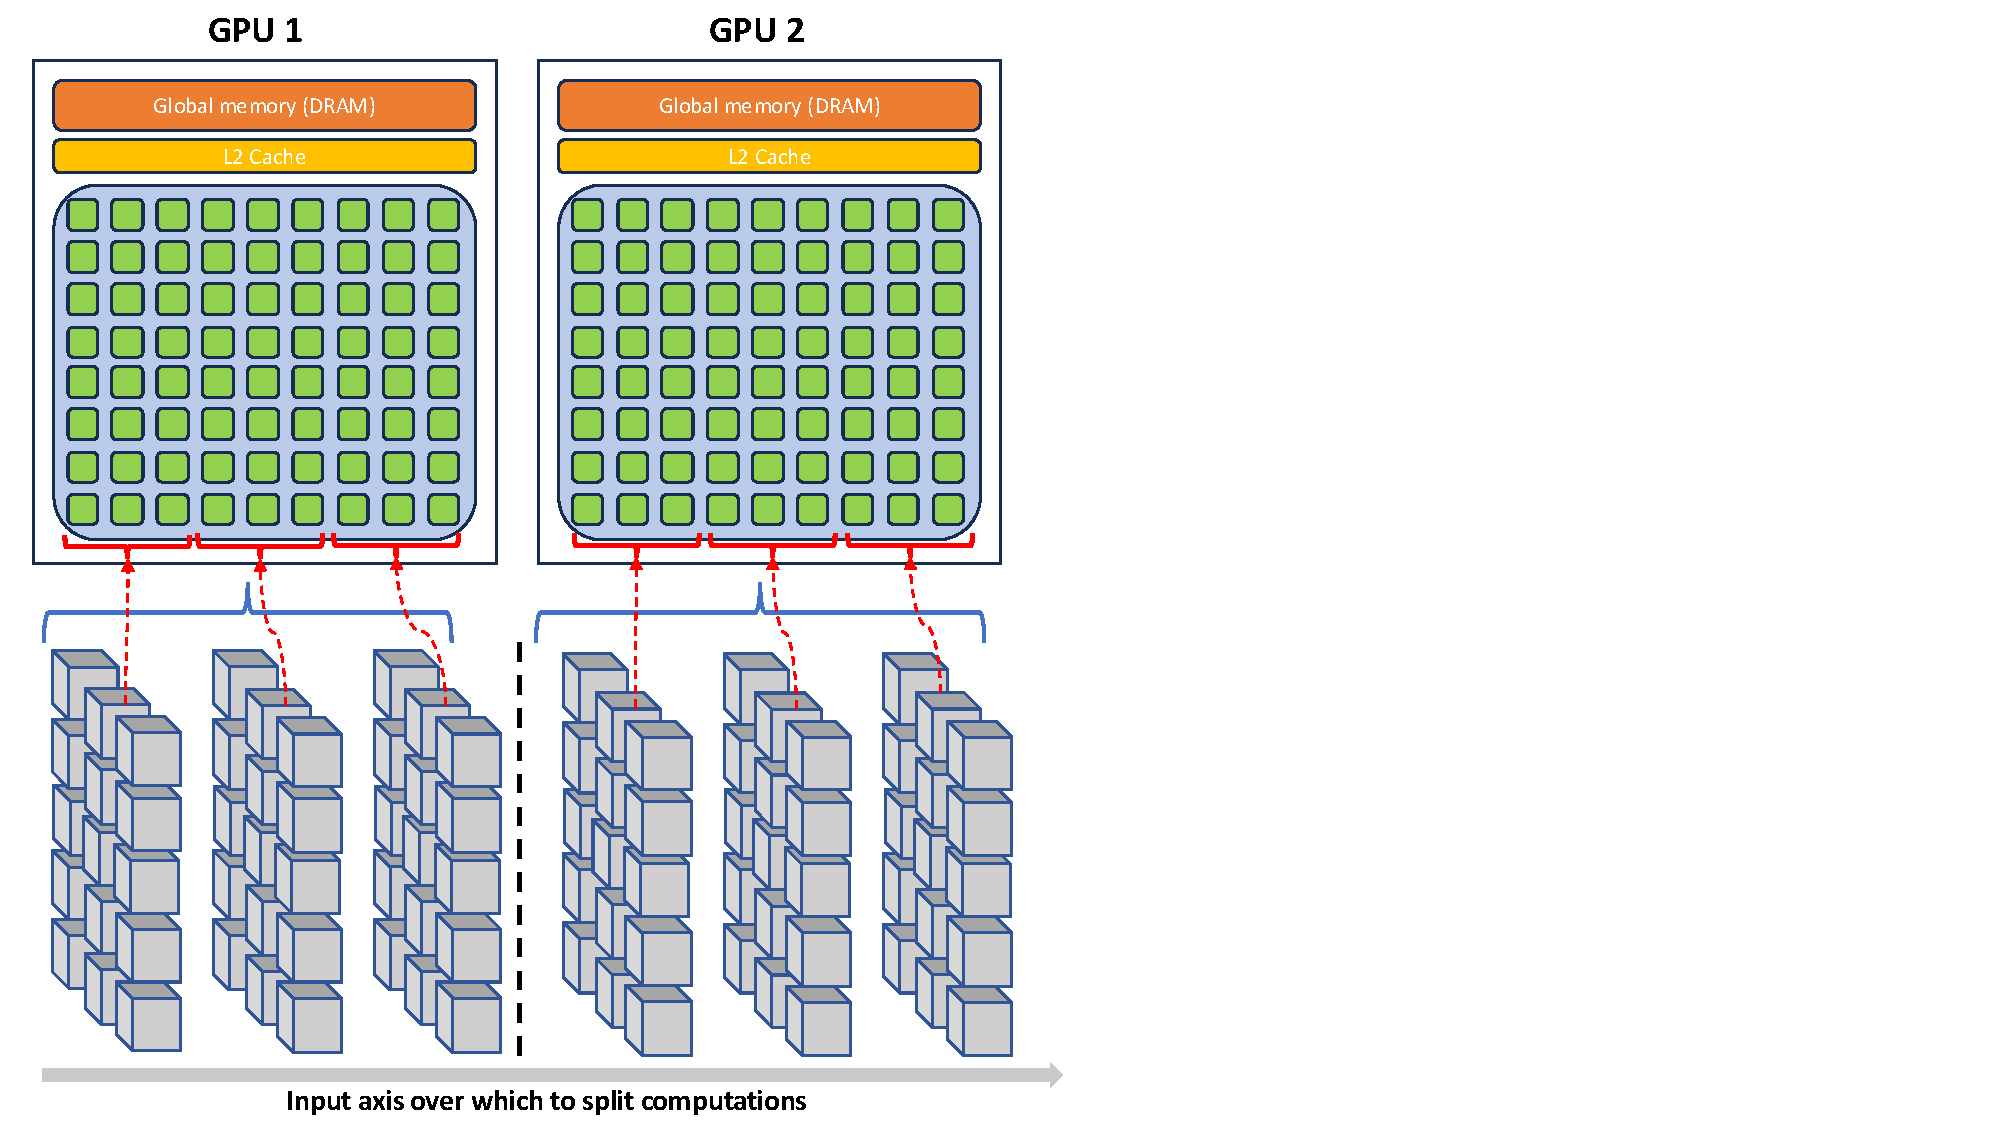
\includegraphics[width=0.65\textwidth]{figs_ext/parallelGPU.pdf}
\caption{\label{fig:org3578035}Input distribution example for multi-GPU runs}
\end{figure}

The inputs are tensors of arbitrary shape from which input data to the solution is built, with the only condition that the first axis being the one over which to run the parallelisation. For the monoeuvre and gust cases below, for instance, the tensor of inputs is a matrix with the second axis being a vector with the combination of flow conditions and gust parameters.   
In the figure we can see each GPU has a global memory and L2 cache, and in addition cores in the GPU are packed into the so-called streaming processors, each with its own registers and L1 caches. The strength of these chips is in the large number of cores, in the thousands, that can run in parallel, thus after the inputs are initially divided, many computations can run in parallel even within each GPU.

\begin{algorithm}[h!]
\DontPrintSemicolon
\Begin{
 \BlankLine
%
\SetKwFunction{Fy}{y\_aeroelastic}
\SetKwFunction{Fyy}{y}
 \SetKwProg{Fn}{Function}{:}{}
  \Fn{\Fy {\texttt{inputs}}}{
   \Fn{\Fyy {\texttt{input}}}{
   ... \;
(nonlinear aeroelastic computation)
\BlankLine
\KwRet \texttt{q, X1, X2, X3, ra, Rab} \;
}
  \texttt{
  yvmap = jax.vmap(y) \;
  q\_multi, X1\_multi, X2\_multi, X3\_multi, ra\_multi, Rab\_multi $\longleftarrow$ yvmap(inputs) \;
  \KwRet dict(q=q\_multi, X1=X1\_multi, X2=X2\_multi, X3=X3\_multi, ra=ra\_multi, Rab=Rab\_multi) \;
  }}

\texttt{
num\_devices $\longleftarrow$ jax.device\_count() \;
mesh $\longleftarrow$  jax.sharding.Mesh( \;
devices=jax.experimental.mesh\_utils.create\_device\_mesh( \;
(num\_devices,)), axis\_names=('x')) \;
inputs = jax.device\_put(inputs, jax.sharding.NamedSharding(mesh, \;  jax.sharding.PartitionSpec('x'))) \;
y\_aeroelastic $\longleftarrow$ jax.jit(y\_aeroelastic) \;
sol $\longleftarrow$ y\_aeroelastic(inputs)
}
    }
\caption{Parallelisation multiple load cases}
\label{org0c0e267}
\end{algorithm}

\subsubsection{Differentiable-parallel load cases}
\label{sec:org7e8990d}
Once a parallel system was in place to compute hundreds of load cases, the next step was to obtain the derivatives of the critical loads coming from the parallel analysis. Since those are calculated using AD, all the operations need to be available in memory.
We encountered two major issues: the memory required for the gust cases was already in the limit of a single device (over 60 GB of RAM), to which the AD normally duplicates the requirement. As the software can now be run on multiple devices, each with its own memory, this is not a completely restrictive factor. The second issue was simply a lack of implementation of the needed collective operations in JAX, as with the maximum function (most of the data generated by such a maximum are zeros not needed anyway). The solution found has been named the Forager Pattern and is depicted in Fig. \ref{fig:org8dc1175}. The code launches many simulations concurrently with the predefined load-cases. The solutions of all these simulations are collected (hundreds of cases, hundreds of nodes, thousands of time steps make for a single field of interest like the stress to have a size of the order of \(10^7\)). A filtering step consists of a selection of monitoring points of interest (nodes in the FEM), and then a double reduction operation in both time and load cases, for example the maximum of the selected field in time and across cases, and the output is a selection of the most problematic load cases according to the predefined metric in the input file. For these critical points the program builds the inputs for the cases previously run in parallel but now with AD and on a much smaller basis, and finally more FENIAX process are spawn for the AD computations. In this way we have created a meta-program that can automatically create programs based on the results, although at this stage is still  very limited on the implemented possibilities.

\begin{figure}[!h]
\centering
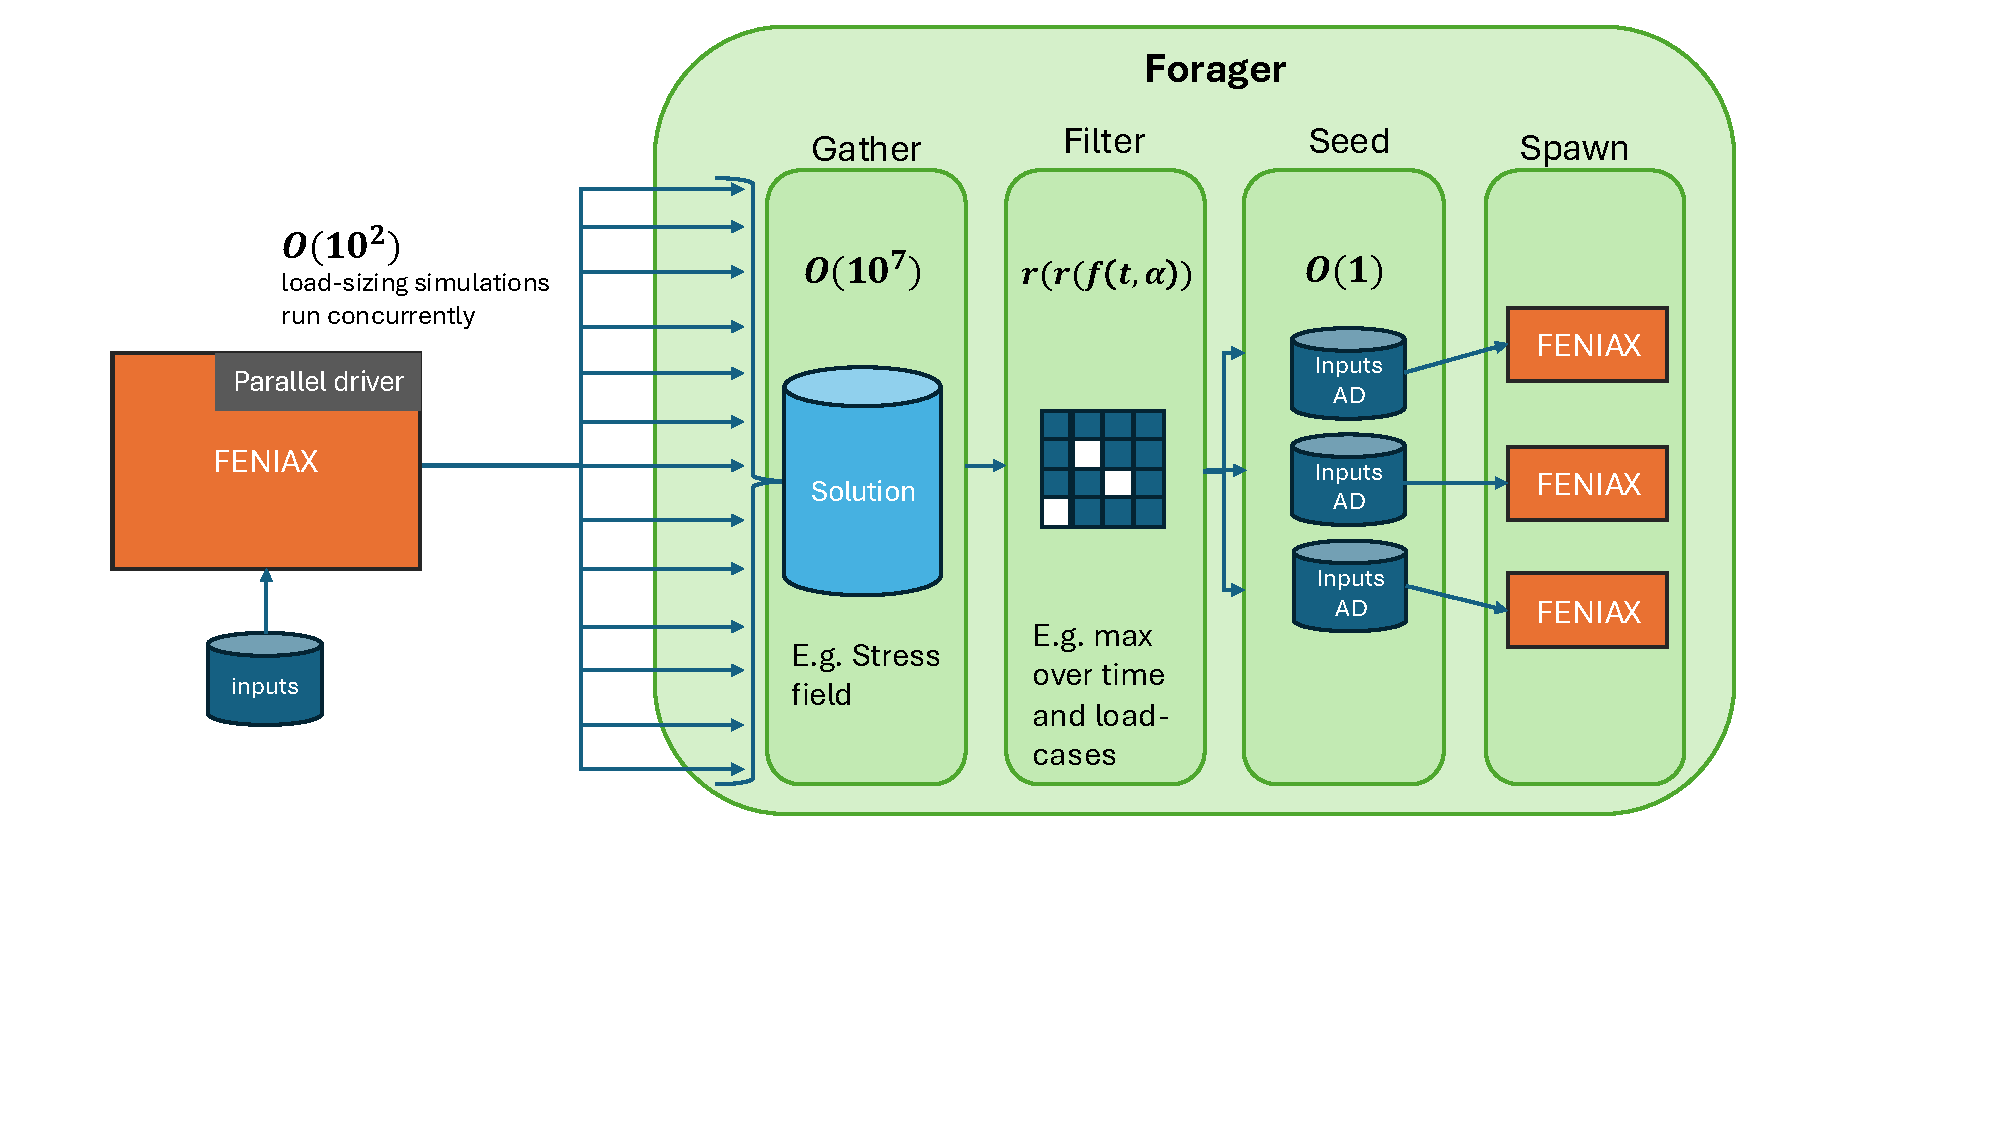
\includegraphics[width=1\textwidth]{figs_ext/forager.pdf}
\caption{\label{fig:org8dc1175}Forager pattern for differentiable-parallel simulations}
\end{figure}

\section{Results}
\label{sec:org0a86af3}
In this section we show the main strengths of our solvers to: a) run a representative aircraft model undergoing very large nonlinear displacements; b) leverage on modern hardware architectures and a parallelisation across devices to unlock problems such as quantifying the uncertainties in the nonlinear response given a loading field that is not fully determinate; c) build load envelopes of static and dynamic aeroelastic simulations.
The University of Bristol Ultra-Green (BUG) aircraft model \cite{STODIECK2018} is the chosen platform to demonstrate these capabilities as it showcases high-aspect ratio wings that are built using a representative GFEM of current industrial models and it is not based on proprietary data. The main components of the aeroelastic model have been presented in 

Structural and aeroelastic static simulations follow, all solved via a Newton-Raphson solver with tolerance of \(10^{-6}\), as well as an assessment of the aircraft dynamics in response to a gust. 
Calculations are carried out on a CPU Intel Xeon Silver 4108 with 1.80GHz speed, 6 cores and a total 12 threads, as well as on an Nvidia GPU A100 80GB SXM. 
\subsection{Uncertainty quantification of nonlinear response}
\label{sec:orge1d2b8c}
uncertainty quantification is performed to the nonlinear response to a loading field that is non-deterministic. Hundreds to thousands of simulations are employed in Monte Carlo type of analysis to resolve for the statistics, for which parallelisation of the independent simulations become critical.
The example resembles the workflow of flight loads and wing stress analysis in an industrial setup.

There will always be an element of uncertainty around the computed loads, and what we show here is how for nonlinear assumptions the statistics need to be computed for every distinct loading. And for this, having a parallisation strategy as the one presented could potentially allow the computation of complex correlations and averages that are more easily calculated under linear assumptions. 

A constant loading force is prescribed along the wings consisting of follower forces in the \(z\)-direction as well as torsional moments, with the characteristic that the force follows a normal distribution \(N(\mu=1.5 \times 10^4 \mu_0, \sigma=0.15 \mu)\) for the vertical forces and \(N(\mu=3 \times 10^4 \mu_0, \sigma=0.15 \mu)\) for the moments. Three scenarios are studied: one in which very large nonlinear deformations are induced with \(\mu_0 = 1\), and two small loading with  \(\mu_0 = 10^{-2}\) and \(\mu_0 = 10^{-3}\).
The distribution of displacements is characterised by means of Montecarlo simulations that run in parallel for a total of 1600 simulations. The modal resolutions consists of 100 modes.
Fig. \ref{fig:org5298a7f} shows the equilibrium for the high loading calculations for two cases out of the 1600. 

\begin{figure}[htbp]
\centering
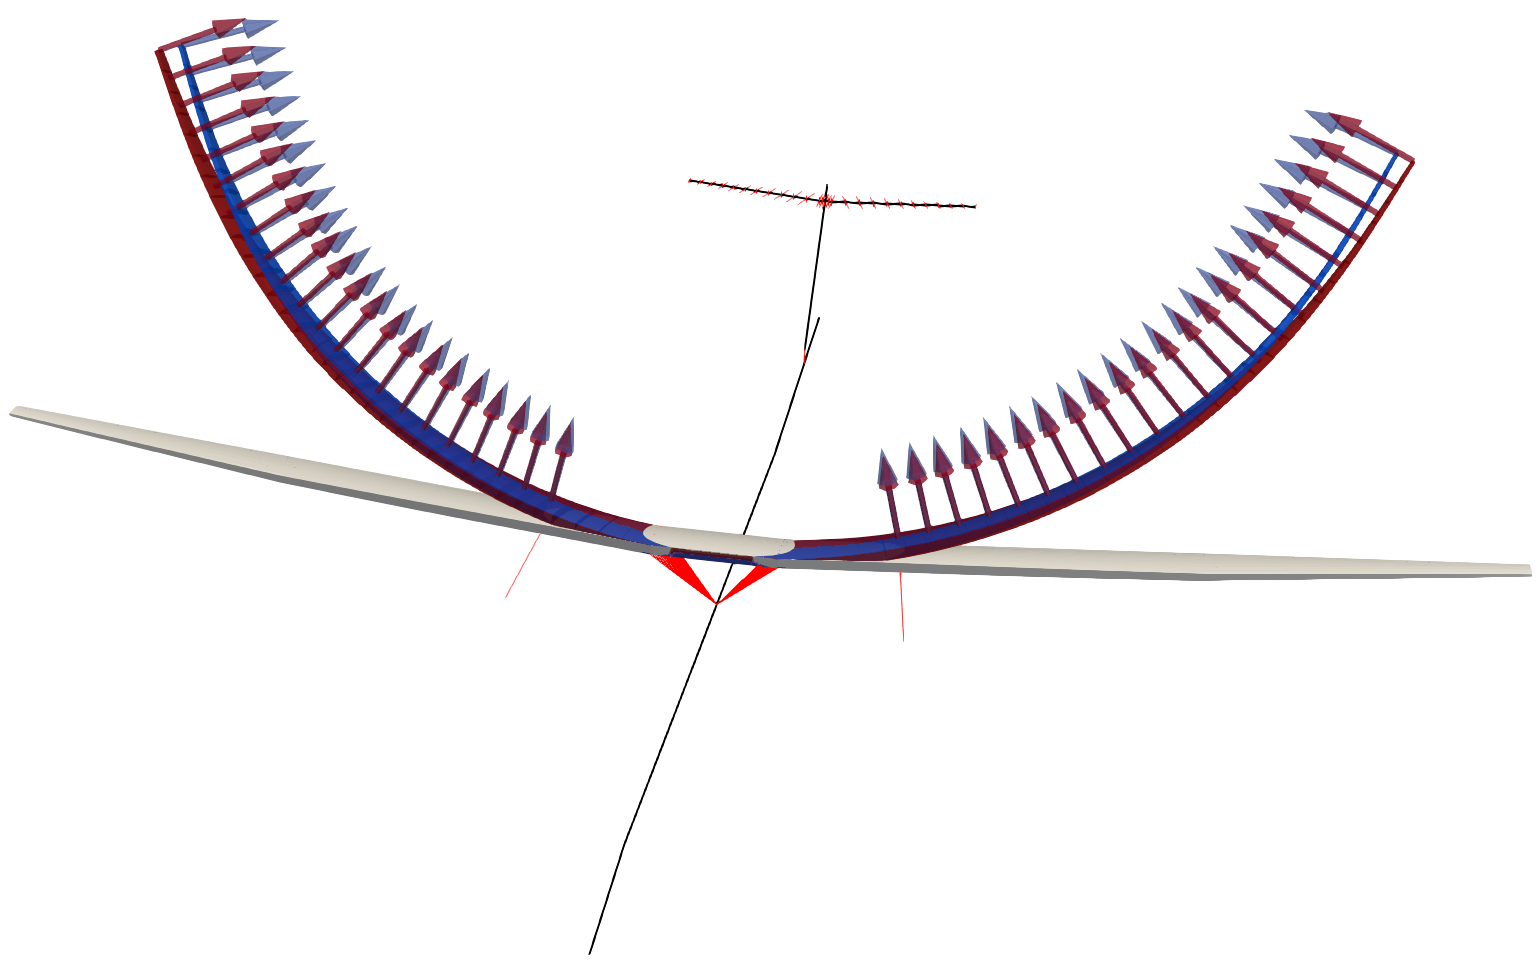
\includegraphics[width=0.8\textwidth]{figs_ext/MC1.png}
\caption{\label{fig:org5298a7f}Static equilibrium for two cases of the random excitation (\(\mu_0=1\))}
\end{figure}

Table \ref{tab:org4a9ec01} shows the statistics gathered from the response
\begin{table}[htbp]
\caption{\label{tab:org4a9ec01}Tip displacement statistics}
\centering
\begin{tabular}{lrr}
Case & Tip displacement mean (m) & Tip displacement std\\[0pt]
\hline
Nonlinear (\(\mu_0 = 1\)) & 11.57 & 1.35\\[0pt]
Linear (\(\mu_0 = 0.01\)) & 0.148 & 0.024\\[0pt]
Very Linear (\(\mu_0 = 0.001\)) & 0.0149 & 0.0023\\[0pt]
\end{tabular}
\end{table}

We can see the statistics of the linear response are fully captured by one example, whereas for a nonlinear response such as \(\mu_0 = 2\), the 1600 simulations would need to be computed again. Table \ref{tab:orgb9e277e} shows the times taken for the nonlinear case. The computation of 1600 independent simulations of Fig. \ref{fig:org5298a7f}, which presents deformations of over 40\% the wing semi-span, in just over a minute, highlights the potential of this methodology in more complex uncertainty quantification problems.  

\begin{table}[htbp]
\caption{\label{tab:orgb9e277e}Computational times uncertainty quantification}
\centering
\begin{tabular}{lr}
Device & Time (sec.)\\[0pt]
\hline
CPU (single) & 16.8 \texttimes{} 1600 = 26880\\[0pt]
CPU (parallel) & 317.4\\[0pt]
GPU & 67.6\\[0pt]
\end{tabular}
\end{table}

\subsubsection{Differentiation of statistical response}
\label{sec:org97aef95}

\subsection{Steady manoeuvre loads}
\label{sec:org1c8afec}
We extend the analysis to a static aeroelastic case for varying angles of attack that represent a manoeuvre scenario. The number of modes used was 100, more than necessary for this type of response, which indicates even faster calculations are possible on this type of analysis. We test the parallelisation by varying the flow density (\(\pm 20 \%\) of the reference density 0.41 Kg/ m\(^3\)) as well and the flow velocity (\(\pm 20 \%\) of the reference velocity 209.6 m/s). 16 different points for both density and velocity make a total number of 256 simulations. The Mach number is fixed at 0.7 corresponding to the reference flow condition values.

Fig. \ref{fig:orgc023faf} illustrates the 3D equilibrium of the airframe at the reference flight conditions. 

\begin{figure}[htbp]
\centering
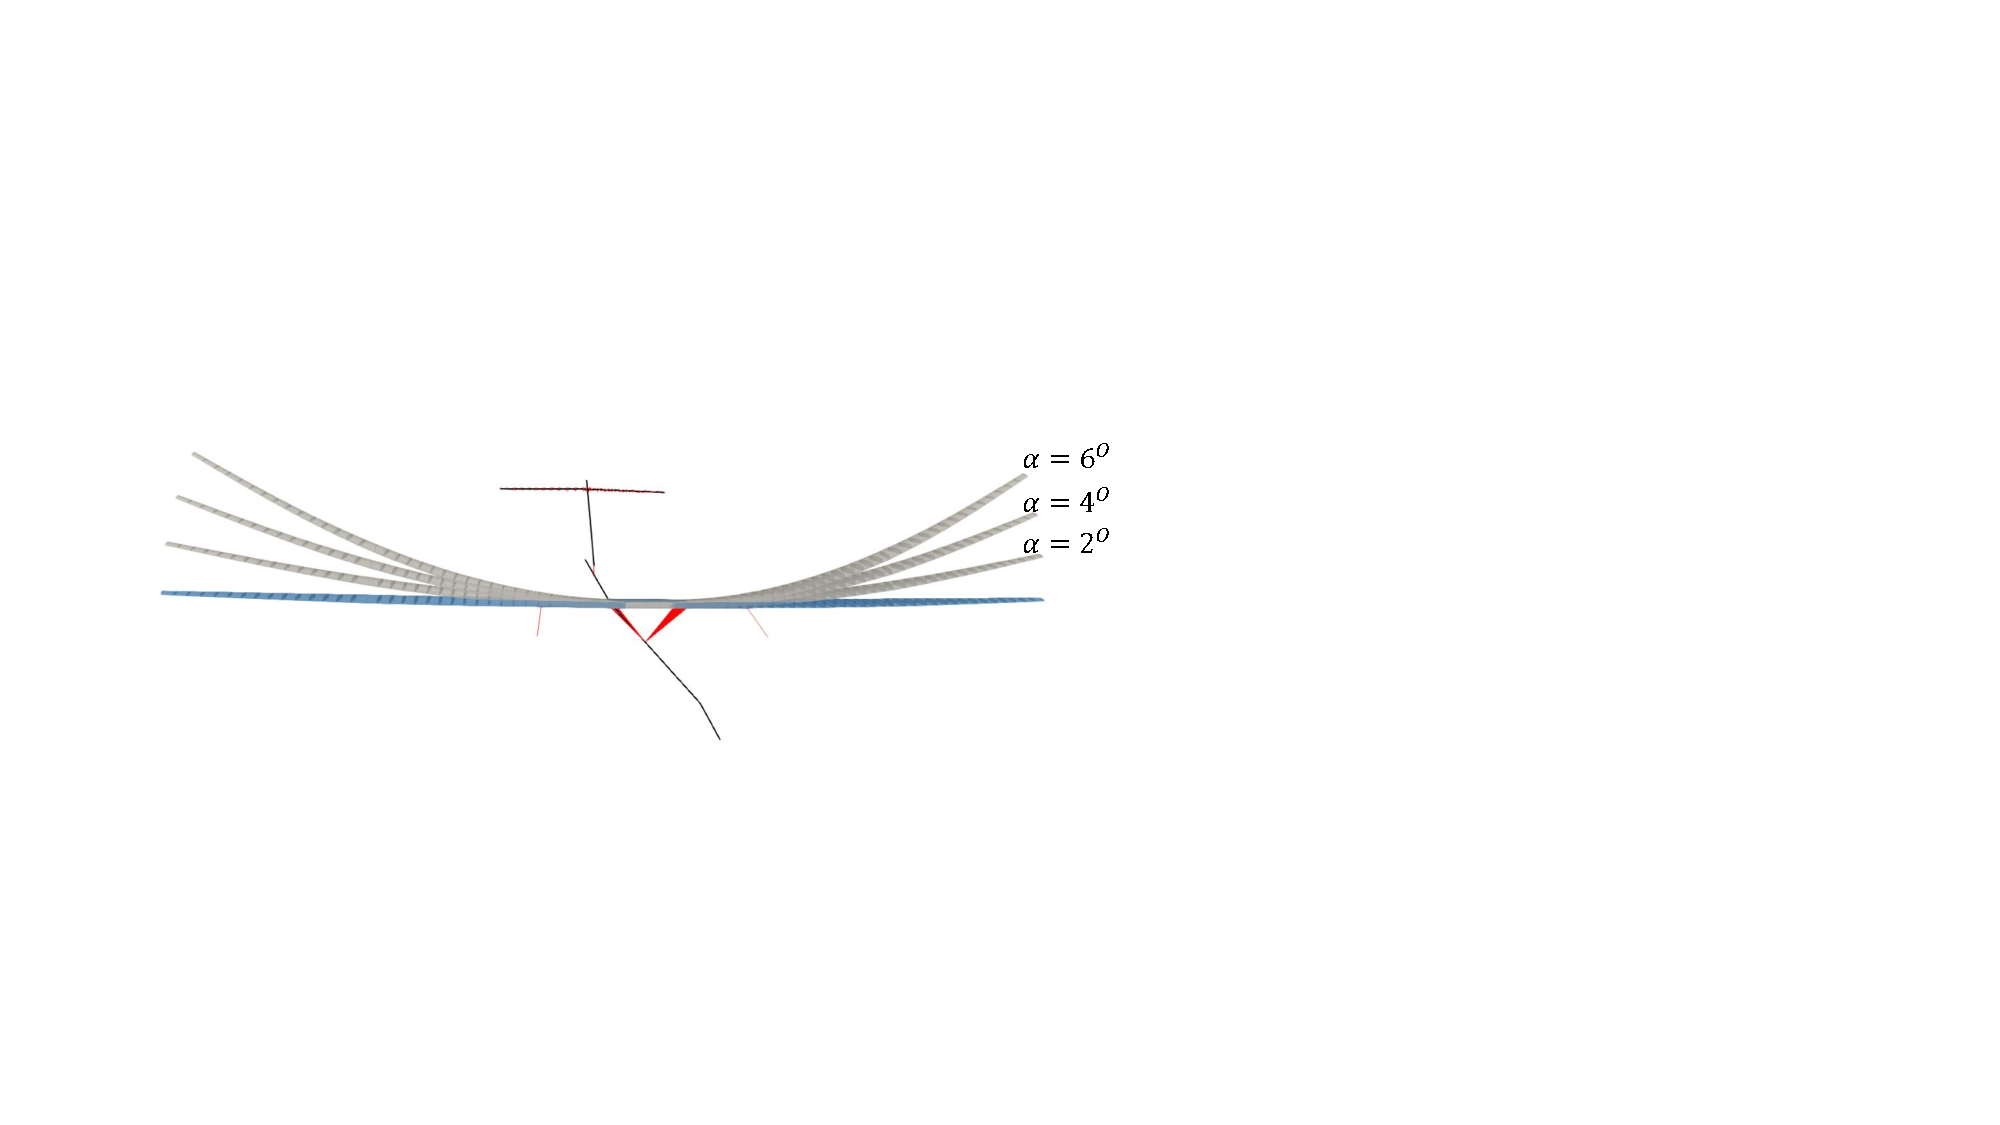
\includegraphics[width=0.95\textwidth]{figs_ext/monoeuvre3D.pdf}
\caption{\label{fig:orgc023faf}Aeroelastic steady equilibrium for increasing angle of attack}
\end{figure}

In Fig. \ref{fig:org2aa5960} the tip of the wing in Fig. \ref{fig:orgc023faf} is plotted for various angles-of-attach (AoA); the tip position falls down the linear projection between the 0 and 1 degrees AoA as expected. This highlights the potential need for geometrically nonlinear aeroelastic tools in future aircraft configurations under high loading scenarios. 

\begin{figure}[htbp]
\centering
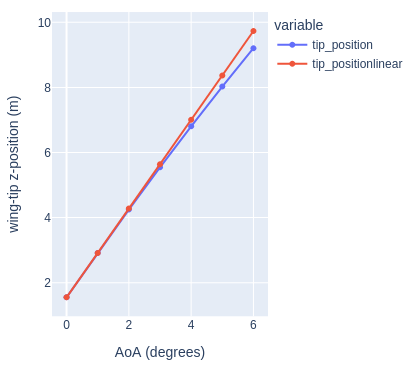
\includegraphics[width=0.65\textwidth]{figs/manoeuvre_wingtip.png}
\caption{\label{fig:org2aa5960}wing tip position for increasing angle of attack}
\end{figure}

Figures \ref{fig:orgd2e3b7b} and \ref{fig:org41f40e0} show the bending-shear-torsion diagrams at the wing-root for all the multiple points computed. Each point is coloured as \(point = \rho_{\infty} / \rho_{max} + u_{\infty} / u_{max}\). The resulting graph is rather predictable with loads increasing with dynamic pressure. A more realistic case could be setup with a trim routine and varying flight condition but the aim of this section was to present the capability to compute multiple manoeuvre loads and compare it with the more interesting case of gust loads as shown in the next section.

\begin{figure}[htbp]
\centering
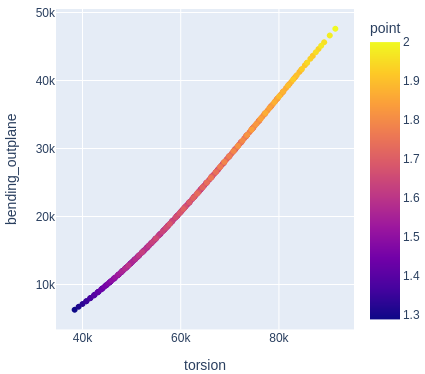
\includegraphics[width=0.5\textwidth]{figs/manoeuvre_bendingtorsion.png}
\caption{\label{fig:orgd2e3b7b}Manoeuvre case, bending-out-of-plane versus torsion}
\end{figure}

\begin{figure}[htbp]
\centering
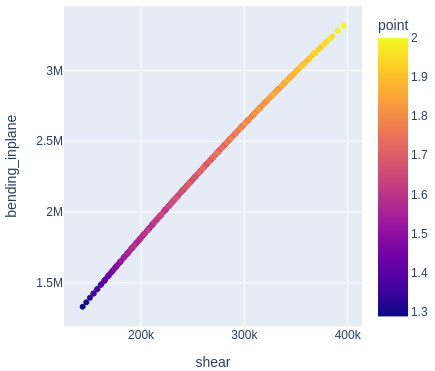
\includegraphics[width=0.5\textwidth]{figs/manoeuvre_bendingshear.png}
\caption{\label{fig:org41f40e0}Manoeuvre case, bending-in-plane versus shear}
\end{figure}

Table \ref{tab:org71806d6} shows the computational times to run these simulations, which shows near no overhead in adding a few hundred of static calculations when moving from the single load case in the CPU to the GPU (nearly 8 seconds to 14 seconds, which amounts for 6 seconds cost when adding an extra 255 cases).

\begin{table}[htbp]
\caption{\label{tab:org71806d6}Computational times for the multiple manoeuvre problem}
\centering
\begin{tabular}{lr}
Device & Time (sec.)\\[0pt]
\hline
CPU (single) & 7.71 \texttimes{} 256 = 1973.8\\[0pt]
CPU (parallel) & 52.8\\[0pt]
GPU & 14.4\\[0pt]
\end{tabular}
\end{table}

\subsection{Dynamic loads at large scale}
\label{sec:orge11333e}
In this final example we perform a dynamic aeroelastic analysis to study the response of the aircraft to multiple 1-cos gusts for varying length, intensity and the density of the airflow. The mach number is kept constant at 0.7. A Runge-Kutta solver is employed to march in time the equations with a time step of \(10^{-3}\) and the total number of modes used was 100. Note the large size of the aeroelastic ODE system: 2 \texttimes{} 100 nonlinear equations plus 5 \texttimes{} 100 linear equations for the aerodynamic states with 5 poles, plus 4 equations for the quaternion tracking the rigid-body motion, for a combined ODE system of 704 equations.  
In addition, a total of 512 gusts cases are run concurrently for all possible combinations of 8 gust lengths between 25 and 265 meters, 8 gust intensities between 1 and 30 m/s, and 8 airflow densities between 0.34 and 0.48 Kg/m\(^3\). This means that \(512 \times 704 = 360448\) equations are being marched in time, in this case for 2 seconds which is enough to capture peak loads. Figs. \ref{fig:org786f0a9}, \ref{fig:org2cc043d} and \ref{fig:org15e0bb1} show the load diagrams for the wing root at the maximum gust intensity of 20, varying 16 gust lengths, \(L\), in the range previously stated and 8 airflow densities,  with the points plotted as \(point = L / L_{max} + \rho_{\infty} / \rho_{max}\). Different load pattern emerge which need further analysis but reflect the importance of running multiple of these simulations to assess the critical loads. 

\begin{figure}[htbp]
\centering
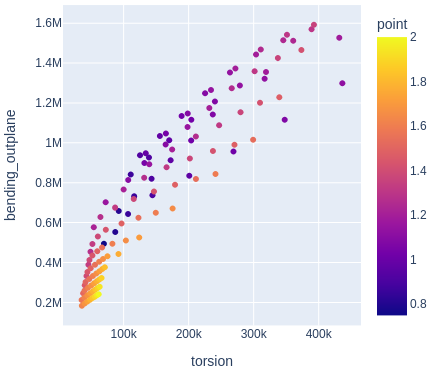
\includegraphics[width=0.5\textwidth]{figs/gust_bendingout_torsion.png}
\caption{\label{fig:org786f0a9}Gust case, bending-out-of-plane versus torsion}
\end{figure}

\begin{figure}[htbp]
\centering
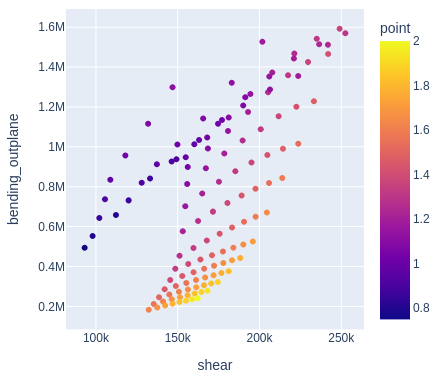
\includegraphics[width=0.5\textwidth]{figs/gust_bendingout_shear.png}
\caption{\label{fig:org2cc043d}Gust case, bending-out-of-plane versus shear}
\end{figure}

\begin{figure}[htbp]
\centering
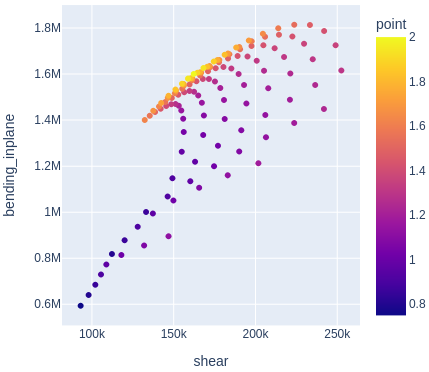
\includegraphics[width=0.5\textwidth]{figs/gust_bendingin_shear.png}
\caption{\label{fig:org15e0bb1}Gust case, bending-inplane versus shear}
\end{figure}

As a validation of the parallelisation, Fig. \ref{fig:orgc341d05} shows the wing tip time evolution for a gust of 150 m length, intensity of 20 m/s and flow density of 0.41 Kg/m\(^3\). Both the results of a single simulation run and that of the 512 parallelised one are shown, which match perfectly.

\begin{figure}[htbp]
\centering
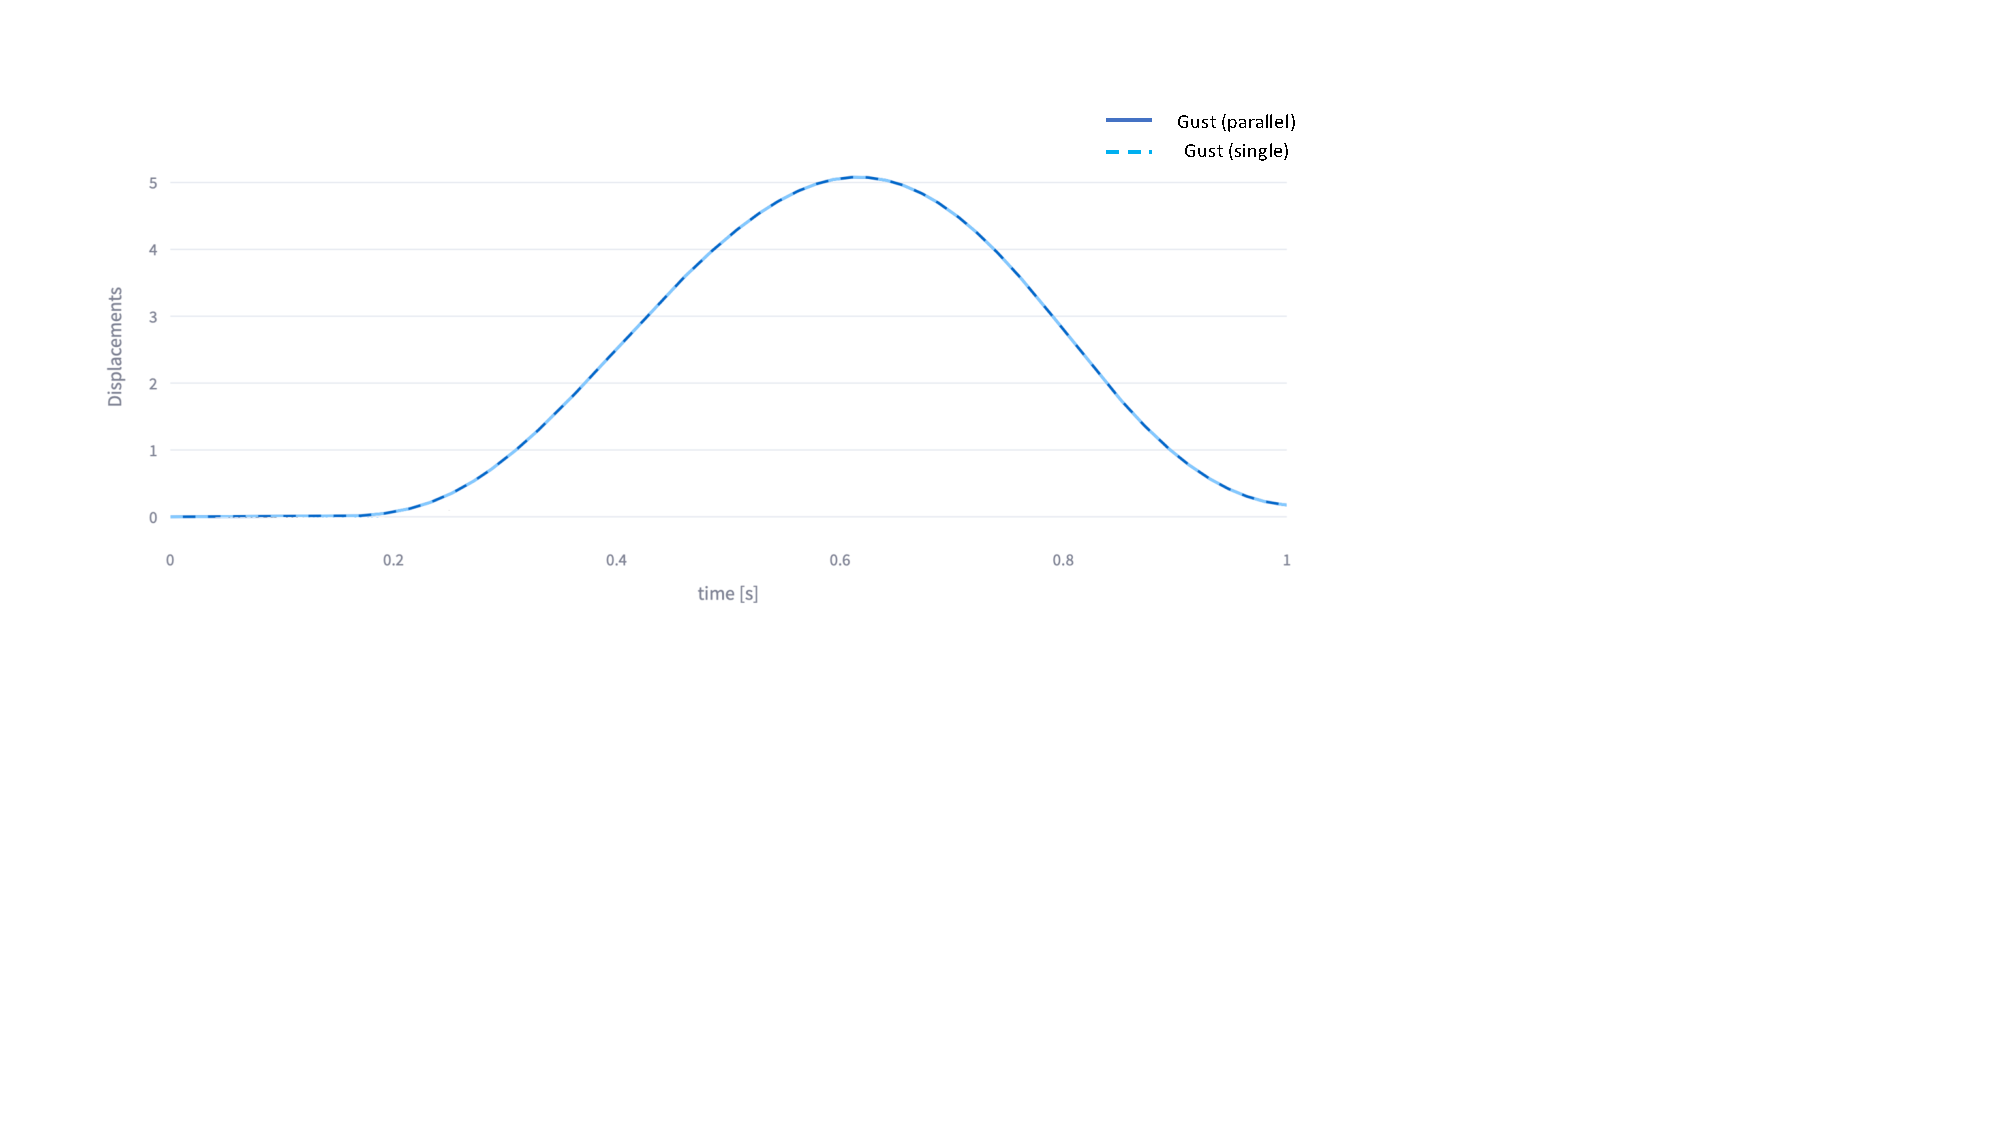
\includegraphics[width=1\textwidth]{figs/bug_gusttip.pdf}
\caption{\label{fig:orgc341d05}\(z\)-component of wing tip response to 1-cos gust excitation (concurrent and single simulation runs).}
\end{figure}

In Fig. \ref{fig:org712993e} the 3D reconstructed flight shape of the airframe is depicted for the simulation in Fig. \ref{fig:orgc341d05}. 

\begin{figure}[htbp]
\centering
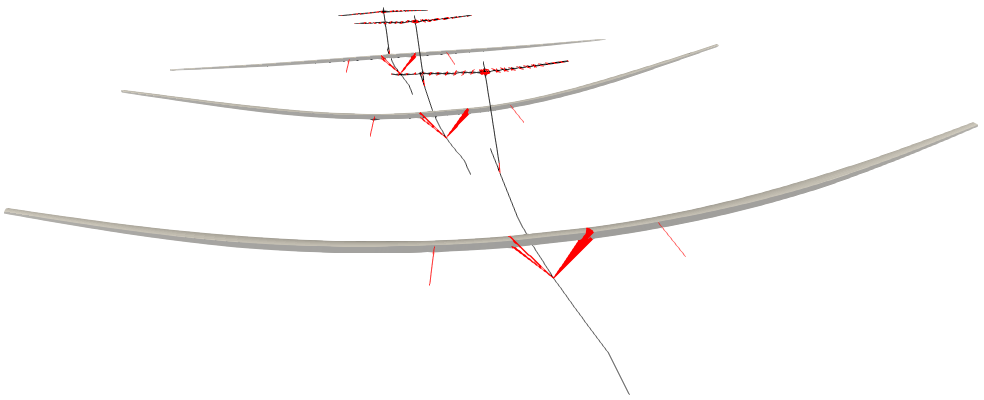
\includegraphics[width=1\textwidth]{figs_ext/Gust3D_3.png}
\caption{\label{fig:org712993e}Full aircraft Dynamic response to 1-cos gust excitation}
\end{figure}

Table \ref{tab:org9cea86c} contains the simulation times of the calculation, which show one order of magnitude increase in performance when running in parallel in the CPU versus a complete single simulation running sequentially, and another order of magnitude when moving from the CPU to a modern GPU.

\begin{table}[htbp]
\caption{\label{tab:org9cea86c}Computational times multiple gust problem}
\centering
\begin{tabular}{lr}
Device & Time (sec.)\\[0pt]
\hline
CPU (single) & 27.8 \texttimes{} 512 = 14233.6\\[0pt]
CPU (parallel) & 922.6\\[0pt]
GPU & 38.2\\[0pt]
\end{tabular}
\end{table}

\subsubsection{Differentiation of dynamic load envelopes}
\label{sec:org19130ec}

\section{Conclusions}
\label{sec:orgb486577}
A modal-based, geometrically nonlinear formulation of the aircraft dynamics has been implemented for multiple load-cases parallelisation in modern hardware architectures. We have applied state-of-the-art techniques and tools employed for large problems in Deep Machine Learning to the computation and prediction of the sizing aeroelastic loads in commercial aircraft, which can expand thousands of simulations. 
Remarkable computational times of under a minute are achieved for 256 manoeuvres varying flow conditions and for 512 dynamic gust responses, including geometrically nonlinear effects in the simulations.
Such a performance potentially unlocks two different applications: uncertainty quantification of the nonlinear aircraft response to a non-deterministic loading and integration of the software in larger multidisciplinary optimisation stuidies.
The former has been demonstrated on a problem where a field of forces with an stochastic component induces very large deformation; it has been shown that while the statistics in the linear response can be easily forecast from one complete experiment, in the nonlinear case a Montecarlo simulation needs to be carried out for each new set of loading scenario.
For the latter, differentiation of the load envelopes via the AD capabilities within JAX will be the next step. Since we are already in the memory boundaries of a single GPU or CPU, this will require the use of multiple devices, for which we have already built the implementation. 
Scaling up the process to include various mass cases, as it is done in industrial scenarios, is also a feasible target. Thus combining prediction of sizing aeroelastic loads that include thousands of cases in commercial aircraft with the computation of their gradients with respect to design variables in a framework for multidisciplinary design optimization.

\newpage

\bibliographystyle{unsrt}

\bibliography{../../../../../Documents/Engineering}
\end{document}
